\chapter{Motion Capture of Rope}
\label{chap:rope}

\noindent
Jie Long, Bryce Porter, Michael Jones. Motion Capture of Rope.

\begin{abstract}
We reconstruct rope motion from passive optical motion capture data using a statistical model without a dynamic model of rope behavior.  Progress in motion capture for faces and cloth has limited applicability to the motion capture of rope because rope is a curved spline rather than a curved surface.  We present clustering, gap repair, and marker swap detection algorithms based on linear interpolation and forward differencing under the assumption that the rope does not stretch.  Indexed marker positions are connected with a spline in each frame to approximate the original rope.  The model produces visually plausible animations of rope motion from data collected for a person interacting with rope.  The method fails when the rope experiences large accelerations that result in motion that is not modeled by forward differencing. 
\end{abstract}

\section{Introduction} 

Motion capture for rope is a challenging problem because rope is a non-rigid body.  The problem is more difficult when the motion of a human character interacting with the rope is also captured in the same scene because, before markers are indexed from frame to frame, it is difficult to separate markers on the actor from markers on the rope.  We present a statistical motion estimation scheme with a clustering model to achieve motion capture of rope from passive optical motion capture data. Our solution consists of novel approaches to clustering and the repair of gaps and swaps, as well as segmenting rope motion from human character motion.

Motion capture of human characters interacting with rope may have applications in the production of computer-generated movies and video games.  Using motion capture data simplifies recording the interaction between characters and ropes while preserving the subtleties of that interaction.  Capturing interactions between rope and characters may be particularly compelling when motion capture is already being used to record character motion.  In this paper, we focus on separating rope motion from actor motion and then reconstructing the motion of the rope.  A variety of existing methods can be used to reconstruct actor motion from motion capture data.  The approach allows reconstructing the interactions between characters and thin, non-rigid bodies.

Prior work on non-rigid motion capture is mainly focused on facial motion (\cite{Lorenzo03,SifakisEftychios2005}) and cloth motion (\cite{MarcusVolker04clothmotion,whiteRyan2007siggraph,PritchardDavid2003,Bhat2003}). Both facial motion and cloth motion aim to build a mesh system for representing the motion of a surface. Motion capture of rope is a fundamentally different problem because rope is more naturally represented as a curved spline rather than as a curved plane (though a curved spline can be used to drive the motion of a plane). 

Human motion capture using a rigid body model (such as \cite{Lou:EHM2010,Wen:2006:MCD,Rajko:2007:RAK,ZordanVictorBrian2003}) is a well-studied area in motion capture but is less applicable to our research as removing the rigid body assumption changes the problem. Worring's \cite{WorringMarcel94measurementof} prior work in reconstruction of a line-shaped object in 3D from several computer images solves essentially the same problem but would require a foreground--background separation step and a sharp image of the rope in each frame.  
 
Our solution reconstructs free motion of rope and ribbon from recorded motion capture data. The captured data consists of an unindexed point cloud of purported marker positions. A marker segmentation algorithm is used to first separate the rope markers from the character so that the two motion streams can be reconstructed individually. A specialized clustering method processes the captured rope motion data and creates motion traces for markers in 3D space. Each cluster represents the motion from a single reflective marker. The clustering process also automatically detects and eliminates most noise. After creating these motion traces, marker swaps are detected and repaired by assuming that the rope does not stretch. Motion capture data marked as noise are revisited and used to fill gaps in marker traces if the data fits existing motion traces without extending the rope length. Small gaps are filled using linear interpolation and big gaps are filled using a structure-based midpoint displacement algorithm. Human character motion can be reconstructed using any of a variety of algorithms for reconstructing human motion from optical motion capture data.  The resulting motion streams containing rope and human motion, respectively, are recombined to recreate the original motion in 3D.

Our contributions are the following: \\
\indent (1) A marker segmentation algorithm that separates rope markers from the character markers.\\
\indent (2) A clustering algorithm to aggregate a point cloud into motion traces for non-rigid ropes and ribbons. \\
\indent (3) Forward differencing to estimate marker locations using previously labeled locations. \\
\indent	(4) A recursive midpoint displacement algorithm for fixing gaps.

These contributions allow us to recreate the interactions of a character with a rope or ribbon from passive optical motion capture data. Side-by-side playback of the resulting 3D motion and video of the original motion show that the captured motion closely matches the original motion.


\section{Related Work} 

The process of reconstructing motion from motion capture data includes data collection, data processing, and model mapping. Commercially available motion capture packages provide tools for creating the motion of a few objects, including human bodies and faces. Current research mainly aims to optimize the usage of collected motion data and to improve the quality of the resulting motion.  However, fundamental issues in the motion capture of non-rigid bodies require additional investigation.  

There are two common approaches to extracting human motion from motion capture data. One is to extract a skeleton model or kinematic model from motion data \cite{Lou:EHM2010,Rajko:2007:RAK}. The other is to predefine the skeleton and to apply motion capture data to animate the predefined skeleton \cite{Wen:2006:MCD,ZordanVictorBrian2003}. Wen \cite{Wen:2006:MCD} uses a least-square optimizing method to match motion capture data to a human skeleton. Zordan \cite{ZordanVictorBrian2003} maps motion capture data to a predefined skeleton using a force-based physical model. In our research, the structure of the rope model is a simple non-branching curve, so we predefine the rope shape and apply our algorithm to automatically map motion data onto the predefined structure.

Liu and colleagues \cite{Liu:tvcj06} take a data-driven approach to completing human motion from a limited set of markers.  A similar approach to rope motion reconstruction would require recording and analyzing many different rope motions, which could then be fit to partial data.  

Instead of a skeleton of rigid parts, non-rigid motion capture focuses on reconstructing a mesh that deforms to match a moving surface such as a face or cloth.  We also investigate non-rigid motion capture, but we focus on curved splines rather than curved surfaces.  

Motion capture for the human face is a well-studied problem.  Approaches that use 3D scans of face geometry \cite{bickel:siggraph07,park:tog06}, a model of the underlying tissue \cite{SifakisEftychios2005}, and displacement maps \cite{Ma:FPS2008,Lorenzo03} have been investigated.  These methods are not adequate for capture of rope motion because modeling deformed surface motion tracks a 2D surface rather than a 1D spline.  In practice a rope can undergo a wider range of motion, (such as coils, loops, and spins) than a face, but markers on rope are visible from all angles, unlike markers on faces, which are visible from only one side of the face.  

Motion capture for cloth is also a well-studied problem.  Prior work has been based on analysis of video of cloth motion, including customized texture patterns \cite{whiteRyan2007siggraph}, optical flow \cite{MarcusVolker04clothmotion}, a stereo pair of images \cite{PritchardDavid2003}, and finding simulation parameters based on video \cite{Bhat2003}.  As with motion capture of the human face, we have posed the motion capture problem for rope differently because rope has a different geometry and range of motions. 

A finite element model can simulate rope motion \cite{jiangWGIJMS1999}, including effects such as tension, shear, bending torsion, contact, and friction. Physical models for involve a parameter system to describe mechanics and structure and can be computationally intensive.

\section{Motion Capture Data} 

We use an optical motion capture system produced by NaturalPoint for recording data.\footnote{The system consists of 12 OptiTrack Flex:V100R2 camera mounted on light poles arranged in a circle with a radius of approximately 2.5 meters.} This section presents the notation used to describe motion capture data. 

\begin{figure*}[tb]
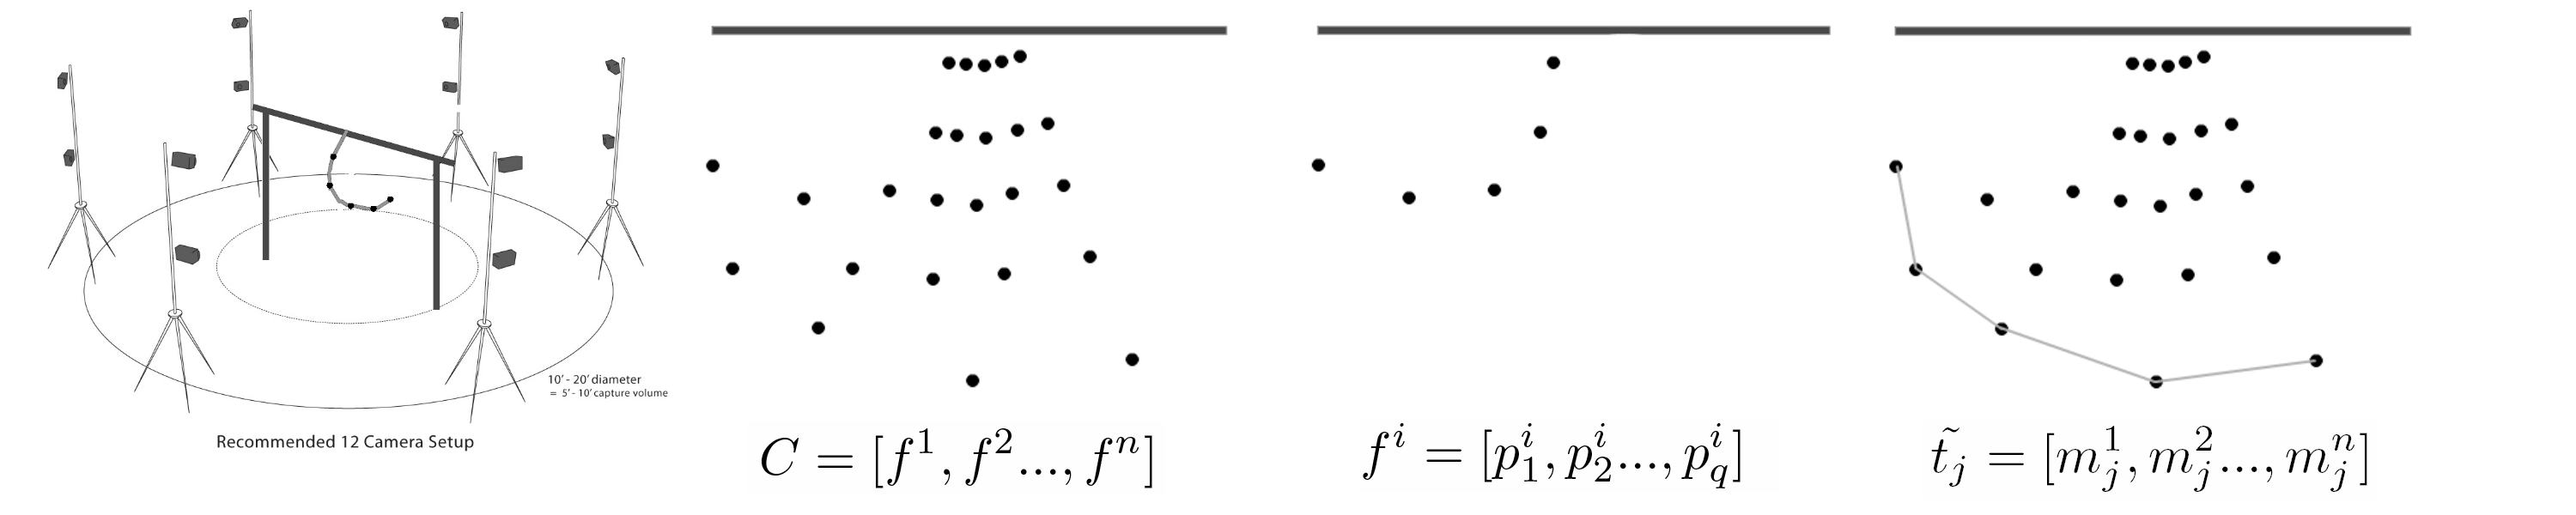
\includegraphics[width=\textwidth]{mocapData1}
\caption{Motion capture setup and notation for describing captured data.}
\label{fig:mocapData} 
\end{figure*}

After the motion capture arena is set up, an actor stands in the center of the arena. There must be enough space on all sides of the actor so that the rope can move freely and still be in the view of the surrounding cameras. Before recording the motion capture session, the actor assumes a T pose while the rope hangs vertically and separate from the actor.  This allows the marker segmentation and rope reconstruction algorithms to be initialized properly. After initialization, the actor can then interact with the rope. 

A motion capture session is $n$ frames of motion capture data:
\[
C=[f^1,f^2...,f^n],
\]
where each frame $f^i(1<i<n)$ consists of an unordered set of $q$ provisional marker locations:
\[
	   f^i=[p_1^i,p_2^i...,p_q^i].
\]
Each $p_j^i (1<j<q)$ denotes the $j$th marker position at frame $i$.  Figure~\ref{fig:mocapData} illustrates these concepts.  The left image shows a motion capture setup with a rope dangling from a pole in the center of an arena.  The next image shows a complete capture session, $C$, consisting of $n$ frames of data.  Next, the marker positions recorded for a single frame $f^i$ are shown.  Finally, the light gray line connects positions in a trace, $t_j$, of the position of a single marker across frames.  

In the following expressions, the superscript $i$ of $p_j^i$ always denotes the frame number. A provisional marker location $p_j^i$ is a triple denoting a 3D position in space. A marker location $m_j^i$ is the location of a specific marker with index $j$ in frame $i$. An initial trace, $\tilde{t_j}$ is an incomplete estimate of the position of a single marker over time and is a list of marker locations. 

\[
\tilde{t_j}=[m_j^1,m_j^2...,m_j^n]
\]

A final trace, $t_j$, is an initial trace after processing to repair gaps and undo marker swap.

In a single trace, a gap is a sequence of frames for which no provisional marker locations were assigned. Gaps are caused by either occluded markers or failure to assign a marker location to a trace.  The position of marker $j$ for which a position is not unknown in frame $p$ is denoted by $m_j^p=\bot$ as a gap. 

Noise occurs when marker locations are created based on transient reflections in the capture arena. Noise that creates motion outside our assumptions about rope motion is automatically detected and eliminated during data processing.

\section{Reconstructing Rope Motion} 

Rope motion can be reconstructed from unindexed marker positions using forward differencing and a novel midpoint displacement algorithm without a physical model assuming that the rope does not stretch. Our aim is to reconstruct rope motion from unindexed motion capture data in the presence of noise and a human actor. 

The main process is shown in Figure \ref{fig:mainProc}.  Markers on the rope are first separated from markers on the human actor so that markers tracking rigid bodies (such as the human actor's bones) can be processed separately from markers tracking non-rigid rope. The separation process is described in Section \ref{segmentation}; that section also shares ideas  from the reconstructing process. The unindexed points remaining after separating rope and actor motion are likely to represent markers attached to rope and are labeled into separate traces using a nearest-neighbor based clustering algorithm. All traces are assigned to a rope structure with a predefined length. Marker swap and gaps in motion traces are detected and repaired using statistical analysis along with the assumption that the rope does not stretch. Provisional marker locations not included in a trace in the first pass are classified as noise but may not be noise. After the first motion reconstruction pass, markers classified as noise are added to existing traces if they match the rope structure and motion. A post-processing step checks rope length and guides another round of processing if necessary. The process iterates until gaps, noise and rope stretching fall below acceptable standards or the algorithm fails to converge. In our research, some data, especially those with swaps and gaps, required two or three rounds of processing, but most of the collected motion capture data required only one round of processing and the algorithm did not converge for data with noise and many large accelerations of the rope.

After all motion capture data are matched into traces while noises and gaps are fixed, a Catmull-Rom spline connects all marker positions and creates a smooth curve among these positions on a rope.

\begin{figure*}[tb]
\begin{center}
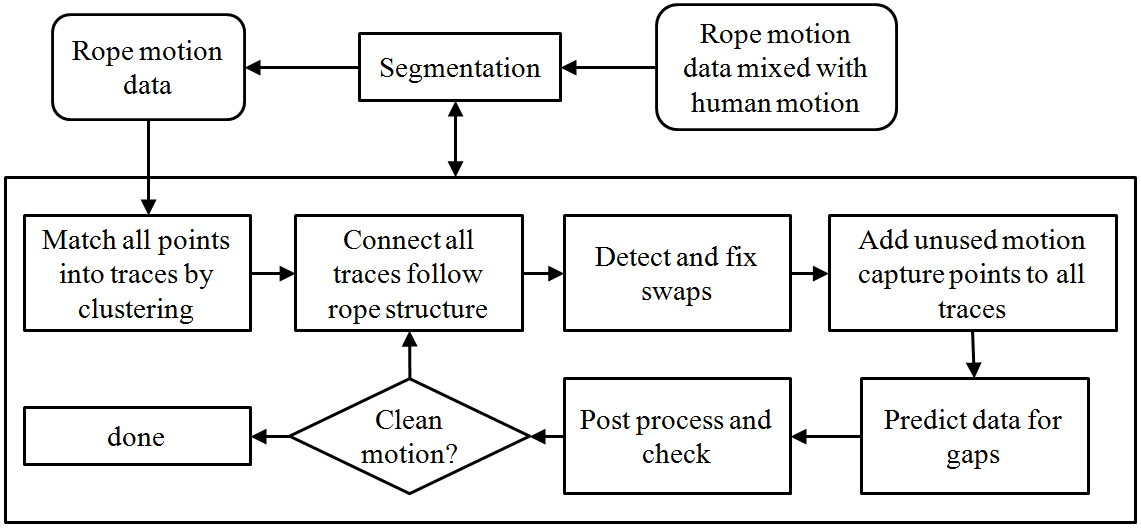
\includegraphics[width=5.5in]{mainProc.PNG}
\end{center}
\caption{Process for converting unindexed marker positions into motion paths.}
\label{fig:mainProc} 
\end{figure*}

\subsection{Clustering Positions into Traces}
\label{secClustering}

For frame $f^i$ and initial trace $\tilde{t_j}$ we attempt to find a provisional position $p_x^i$ that is a good match for $\tilde{t_j}$ in that frame.  If no match is found, we set $m_j^i=\bot$.
\[
m_j^i=\left\{\begin{array}{ll}p_x^i & \ \ \ \ \ \mbox{if $p_x^i$ is a good match for trace $\tilde{t_j}$ in frame $f^i$}\\
\bot & \ \ \ \ \ \mbox{otherwise}\end{array}\right.
\]

First, a small portion of the capture session with little or no movement is processed in order to find the number and locations of markers. Next, a second round of clustering assigns provisional marker positions across all frames to zero or one of the identified traces.  Positions not assigned to a trace are marked as noise and may be added to a trace later.  Each round of clustering is discussed in detail below.  

\subsubsection{First Round of Clustering}
The first round of clustering is performed on a stationary prefix session in which the markers remain stationary for approximately one second. This is similar to capturing a T pose during a motion capture session with a human actor.  

Two parameters, $\gamma$ and minPoints, are predefined. Parameter $\gamma$ is a 3D vector of the maximum allowable movement range for a marker during the stationary prefix.   Parameter minPoints is a threshold for the minimum number of provisional marker locations that must be assigned to a trace for that trace to be retained in the next round. A trace set $T$ is initialized by separate initial traces $\tilde{t_j}$ as 
\[
T={\tilde{t_1},\tilde{t_2},\tilde{t_3}...}. 
\]

In frame $i$, a position $p_x^i$ is appended as a marker location to trace $\tilde{t_j^i}$ when it is the closest provisional marker location to the average position of all the previous marker locations in a trace and it is within the threshold $\gamma$. If no such provisional location exists for a trace $\tilde{t_j^i}$, a gap $\tilde{t_j^i}=\bot{}$ is marked for trace $j$ in frame $i$. When a provisional marker location $p_x^i$ is not appended to any trace, a new trace $\tilde{t_j^i}$ is initialized with $\tilde{t_j^i}=p_x^i$. After all provisional marker locations are processed, traces which have fewer recorded positions than the threshold minPoints are discarded and the positions are marked as unused data for future analyses. 

\subsubsection{Second Round of Clustering}

The second round of clustering matches markers to traces using forward differencing (FD) to predict future marker locations. FD with order $s$ predicts an expected position $D_j^i$ for trace $\tilde{t_j^i}$ in frame $i$. Differencing $\Delta_j^s$ is computed with order $s(s>0)$ for trace $\tilde{t_j^i}$ from the previous frames $(i-s)$ to $(i-1)$:

\begin{equation}\label{eq:1}
\Delta_j^s=\Delta^sm_j=\sum_{w=1}^s(-1)^s\left(\begin{array}{c}s\\w\end{array}\right)m_{j+s-w}.
\end{equation}

After getting the differencing values $\Delta_j^s$, the predicted new position $D_j^i$ for trace $j$ in frame $i$ is estimated as 
\begin{equation}\label{eq:2}
D_j^i=\sum_{w=0}^s\left(\begin{array}{c}s\\w\end{array}\right)\Delta_j^wm_{j}^{i-w}.
\end{equation}

The predicted position $D_j^i$ preserves motion continuity from the previous $s$ frames in trace $t_j$. Finding a new provisional marker position in the neighborhood of the predicted position $D_j^i$ is more precise than searching in the locus of the average position because the expected position varies with velocity and acceleration.  

However, large accelerations can result in a predicted marker position that is at a different location than the actual marker.  If the actual marker lies outside the neighborhood of the predicted position then the marker will be missed, a gap will be created in the trace, and the marker position will be marked as noise.  Later, after repairing gaps and swaps, it may be possible to insert the missing marker position into the trace.   

\begin{figure}[tb]
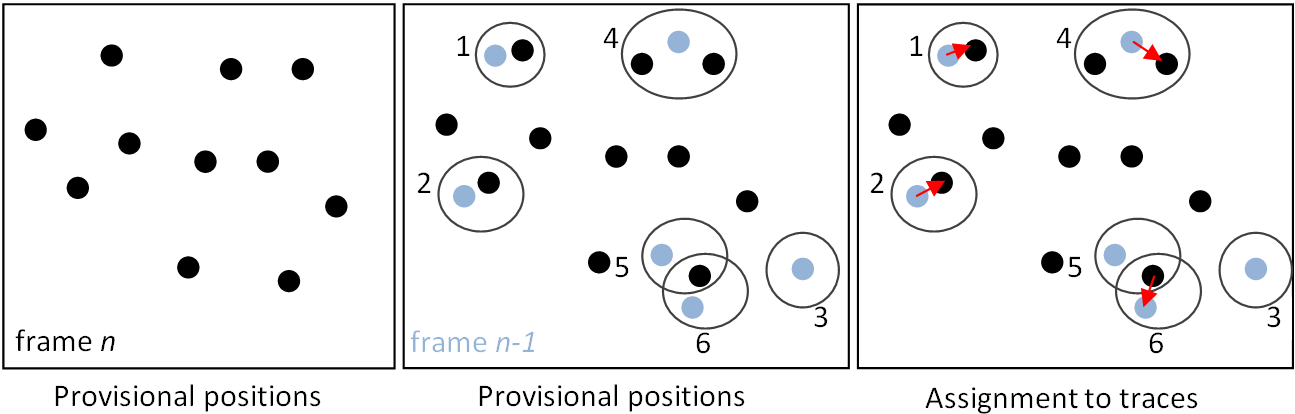
\includegraphics[width=\columnwidth]{ClusterProc.png}
\caption{Clustering process for the second round.}
\label{fig:ClusterProc} 
\end{figure}

Figure~\ref{fig:ClusterProc} illustrates the clustering process. The image on the left shows the provisional marker positions in $f^i$.  FD on markers 1 through 6 from $f^{i-s}$ to $f^{i-1}$, where positions of markers 1 through 6 from $f^{i-1}$ are shown in light gray, is used to identify likely positions of markers 1 through 6 in $f^i$.  These likely positions are called neighborhoods and are contained in the gray circles in the middle image. Next, for all marker positions $m_j^i$ in the neighborhood of $D_k^i$  compute:

\begin{equation}\label{eq:3}
\tilde{t_k^i}=m_j^i=min_{\forall{p_x^i}\forall{D_y^i}}\left\|p_x^i-D_y^i\right\|.
\end{equation}

A provisional marker location $p_x^i$ is appended to trace $\tilde{t_k^i }$ if $p_x^i$ is the nearest provisional marker location in the neighborhood $D_k^i$ predicted from trace $\tilde{t_k^i}$.  This is shown on the right side of Figure~\ref{fig:ClusterProc} as one of the provisional markers is assigned to traces 1, 2, and 4. In each case, the provisional marker location is assigned to a trace that has the nearest neighborhood $D_k^i$ to the location.  If no such $p_x^i$ lie within the forward differencing estimation then $\tilde{t_k^i}=\bot$. In Figure~\ref{fig:ClusterProc}, trace 3 is assigned to $\bot$ because no provisional locations lie close enough to the position of trace 3 from $f^i$.  A provisional marker location $p_x^i$ might be mapped to more than one trace---as is the case for traces 5 and 6 in the figure. In this case, the closest trace keeps the provisional marker location $p_x^i$ while the others are marked as having a gap. In this case, trace 6 is closer to the shared position and trace 5 is marked with a gap. If a provisional marker location $p_x^i$ is not clustered with any trace then that position is marked as unused data. The remaining black dots in the right side of Figure~\ref{fig:ClusterProc} are marked as unused data and may be assigned to traces later, which is discussed in Section ~\ref{sec:addUnusedSec}.  

Figure~\ref{fig:SecCluster} demonstrates a trace graph for 5 dangling ropes instrumented with 5 markers each. The left image is before clustering and the right is after. All traces are painted in different colors. Black circles indicate the stationary positions of each marker. Noise and unused data are detected but not shown in the image of the reconstructed traces on the right. 

\begin{figure}[tb]
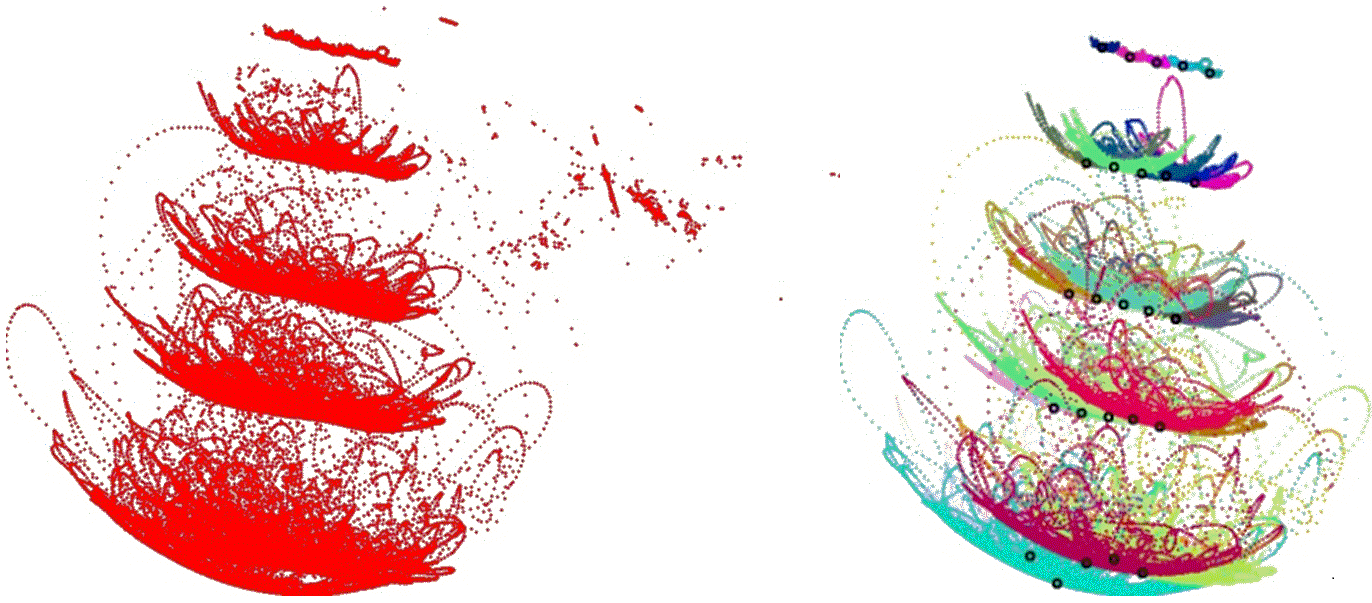
\includegraphics[width=\columnwidth]{SecCluster.png}
\caption{An input point cloud and clustering result.}
\label{fig:SecCluster} 
\end{figure}

\subsection{Swaps}

Marker swap occurs when marker positions are assigned to the wrong trace.  In our data, marker swaps occur at a rate of about one swap per thousand frames of data.  While swaps are uncommon, swaps lead to visually implausible animations, as the rope appears to twist and bend unnaturally.  In many cases, swaps lead to the appearance of the rope stretching. This is the key to detecting such swaps. A rope with length greater than the initial stationary length is called a stretched rope and likely indicates a marker swap.  

A segment is the span of rope between any two markers on a single rope. Stationary marker positions from the first round of clustering are denoted $\bar{m_x}$ and $\bar{m_y}$. With a distortion factor $\alpha$ for length error tolerance, a rope segment between markers $m_x$ and $m_y$ is considered stretched if
\begin{equation}
\left\|m_x^i-m_y^i \right\|>\alpha*\left\|\bar{m_x}-\bar{m_y}\right\|.
\label{eq:strech}
\end{equation}
The distortion factor $\alpha$ is small enough to detect swaps before they are visually significant. We set the value of $\alpha$ in [0.1,0.15]. 

We implemented two approaches for finding rope stretching: a case-based approach and brute force. The case-based method only checks rope length when there is a reasonable chance of swapping while the brute force approach checks rope length in every segment in every frame.
 
In the case-based approach, we collect candidate swapping points based on two assumptions: (1) when the distance between any two provisional marker locations is smaller than a threshold $minDist$ and (2) after a gap whose length is bigger than a threshold $maxGapLen$. After collecting all candidate swapping points, the segment length at a candidate swapping frame is checked using equation \ref{eq:strech}. After two markers approach in space, the following $N$ frames have higher probability of containing a swap because the clustering-based labeling process might swap positions.  Therefore, segment length is checked the $N$ frames after markers pass in close proximity.  A related segment is a rope segment that contains candidate swapping points.  A swap of two candidate points is detected and repaired if the potential swapping satisfies two requirements: (1) before the swap, both lengths of related rope segments are stretched, and (2) after the swap, at least one of these lengths is corrected.

In the brute force method, the rope length is checked in each frame using equation \ref{eq:strech} with a distortion factor $\alpha$.  When rope length is stretched in a frame, we try all permutations for all marker positions for all ropes in a scene.  Swap repair stops when all rope lengths are not stretched or when all permutations have been checked.  However, in the worst case, the number of permutations is in the order of $n!$, where $n$ is the number of marker locations. That makes this approach infeasible in most cases.

\subsection{Gaps}
\label{sec:Gaps}

Given a trace, a gap is a sequence of frames in which recorded marker positions were not assigned to that trace.  Gaps are repaired by filling gaps with estimated locations. A small gap has less than five continuous missing frames. Small gaps are fixed by linear interpolation. Fixing a large gap uses assumptions about rope shape, statistical characteristics of the marker and the movement of other markers on the same rope.  This section focuses on repairing large gaps.

A gap session is a span of time in which multiple traces have gaps. During a gap session, multiple traces might have gaps with different durations. Smaller gaps and gaps in traces with small ranges of motion (if any) are repaired first.

\begin{figure*}[tb]
\center
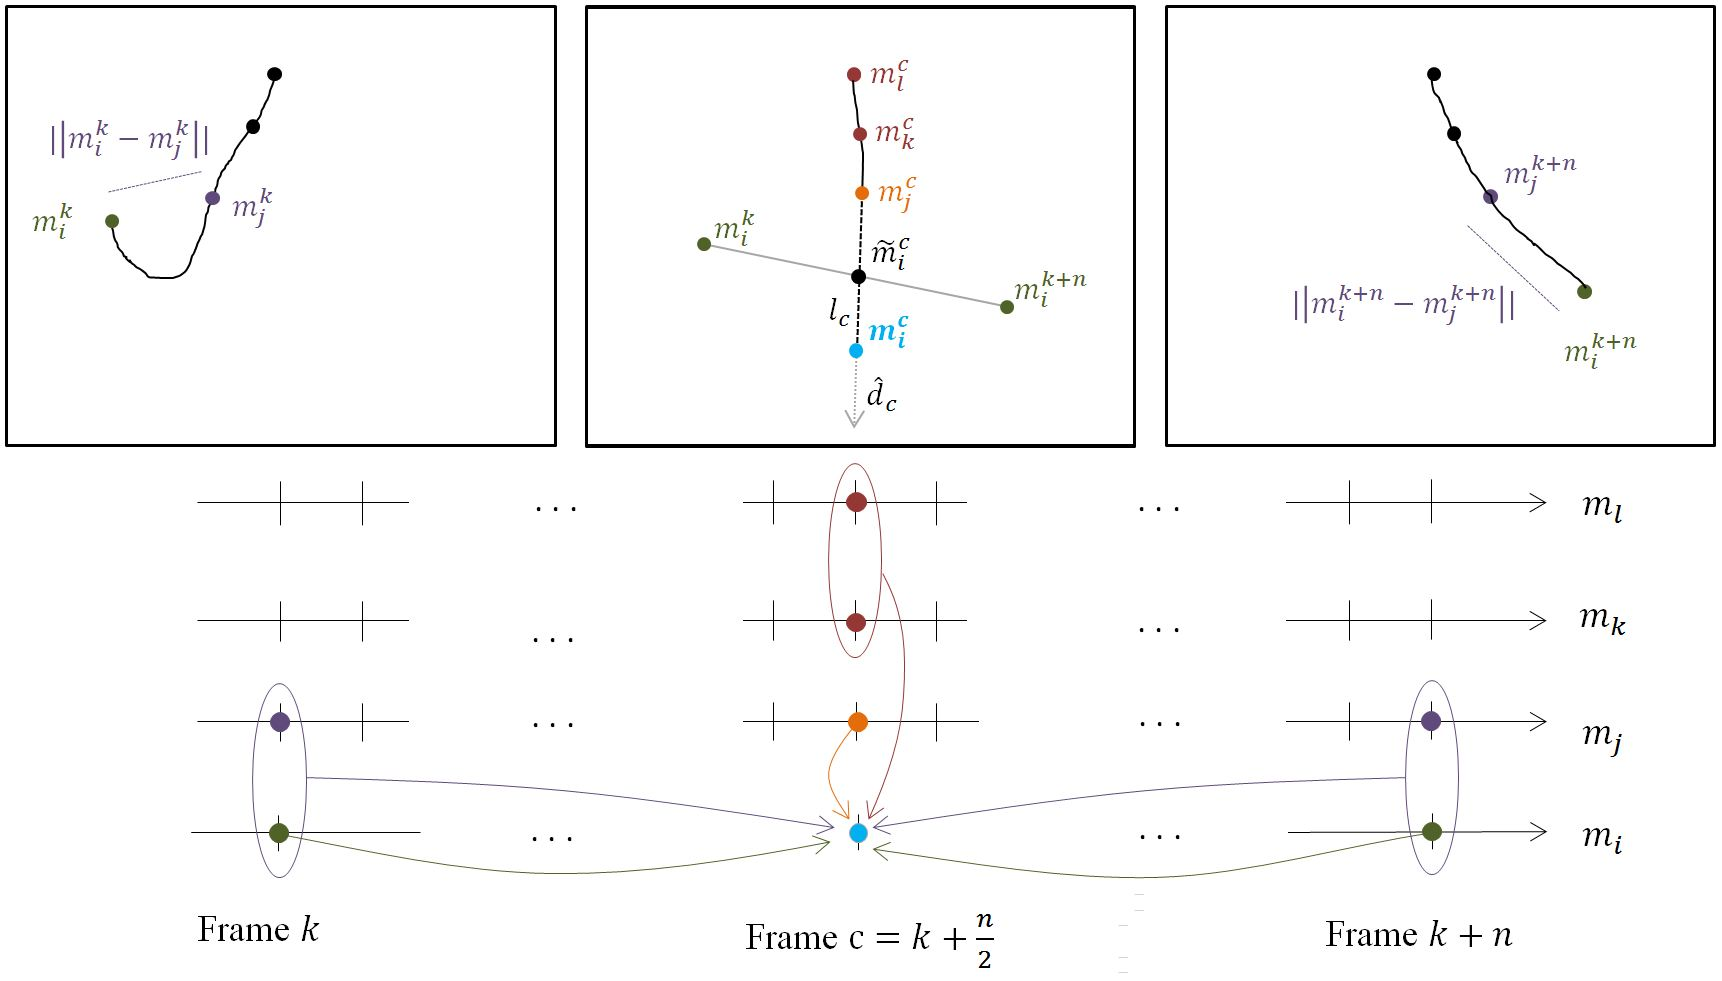
\includegraphics[width=1.0\textwidth]{filling-gaps-2.jpg}
\caption[Estimate the position of marker.]{Estimating the position of marker $m_i$ in the center frame of a long gap using the positions of markers $m_j$, $m_j1$, and $m_j2$.}
\label{fig:gapFix} 
\end{figure*}

A recursive midpoint displacement method estimates marker positions through large gaps. This process is shown in Figure~\ref{fig:gapFix}. Suppose the trace of marker $m_i$ includes a gap from frames $k$ to $k+n$ and that the trace of nearby marker $m_j$ is complete over the same span.  Marker $m_j$ is adjacent in the sense that it lies next to, or near, marker $m_i$ on the rope segment.  Figure~\ref{fig:gapFix} contains rope positions in the top series of frames, and timelines at the bottom of the figure show which marker positions in which frames are used to estimate the position of marker $m_i$ at the frame $k+n/2$ in the middle of the gap.  Marker locations in the top series of frames and the timelines are color-coded.  The process involves estimating the distance between $m_i$ and $m_j$, estimating the position of $m_i$, and then estimating direction from $m_j$ to $m_i$.  These estimates are generated from known marker positions in frames $k$, $k+2$ and the midpoint frame.  

The estimated distance between known markers for the segment at the middle frame, $l^c$ (where $c=k+n/2$), is computed by averaging the segment length between $m_j$ and $m_i$ (shown in purple in the figure) starting in frame $f_k$ and ending in frame $f_{k+n}$. 
\begin{equation}\label{eq:6}
l^c=\frac{\left(\left\|m_i^k-m_j^k\right\|+\left\|m_i^{k+n}-m_j^{k+n}\right\|\right)}{2}
\end{equation}   
The preliminary location of $m_i$ in frame $c$, which is denoted $\tilde{m_i^c}$, is the average of the locations of $m_i$ at the start and end frames. 
\begin{equation}\label{eq:7}
\tilde{m_i^c}=\frac{m_i^k-m_i^{k+n}}{2}
\end{equation}
The position of $m_i$ at the start and end frames is shown in green in Figure~\ref{fig:gapFix}. 

Next, the direction from $m_j^c$ to $m_i^c$ is estimated using the weighted sum of the direction from $m_j^c$ to $\tilde{m_i^c}$ and the direction between two other nearby markers $m_{j1}^c$ and $m_{j2}^c$ (shown in red in Figure~\ref{fig:gapFix}).   
The direction $\hat{d^c}$ is given by 
\begin{equation}\label{eq:8}
\hat{d^c}=Norm\left[\alpha*\left(m_j^c-\tilde{m_i^c}\right)+\beta*\left(m_{j1}^c-m_{j2}^c\right)\right],
\end{equation}
where $\alpha$ and $\beta$ are weighting parameters.   

Finally, the location of marker $m_i^c$ in frame $c$ is determined by moving a total of $l^c$ units along the normalized vector $\hat{d^c}$ starting at known marker location $m_j^c$:
\begin{equation}\label{eq:9}
m_i^c=m_j^c+l^c\hat{d^c}.
\end{equation}
The new position is shown in blue in Figure~\ref{fig:gapFix}. 

The midpoint displacement method proceeds recursively and fills data in all the gaps in the gap session. When length of a sub-session gap is fewer than 5 frames, it will be fixed using linear interpolation. 

\subsection{Add Unused Data}
\label{sec:addUnusedSec}

The unused data are revisited and added to existing traces if applicable. The nearest unused provisional location $p_y^{i}$ to a marker location $m_x^{i\pm1}$ in the neighboring previous or next frame fills a gap location $m_x^i = \bot$ if 
\begin{equation}
m_x^i=p_y^i=min_{\forall{m_x^i}\forall{p_y^i}}\left\|p_y^i-m_x^{i\pm1}\right\|,
\label{eq:addUnused}
\end{equation}
where $y\in{y_1,y_2,...y_z}$ and ranges over unused locations. 

The segment length resulting from using the closest provisional location $p_u^i$ is evaluated using equation~\ref{eq:strech}. If the segment is not stretched and equation \ref{eq:addUnused} is satisfied, the unused provisional location will be added in a trace to replace a gap $m_x^i$.

The process is repeated over the entire session. When there is a gap, the left and right ends of the gap are processed first because there are data available in the neighboring previous or next frames. This process is repeated for all gaps until no more unused data is added to a gap.

\subsection{Separate Rope Markers from Actor Markers}
\label{segmentation}

Rope motion captured with a human actor is separated from the actor's motion.  The segmentation is an important step in our method for recreating animation of an actor interacting with rope.  Rope markers are separated from markers on the actor after grouping markers into traces across frames.  The clustering method used to group markers is identical to the clustering method described above.   Alternatively, it may be possible and more desirable to separate rope and actor markers by tracking the actor skeleton as a collection of rigid bodies and classifying the remaining marker positions as rope markers.  

After the segmentation, rope motion is reconstructed from purported rope marker positions by repairing gaps and swaps and then adding unused markers as described previously.  To initialize rope marker locations, a user makes a simple selection of all and only the markers that belong to the rope, as shown in Figure~\ref{fig:SegInit}. 

\begin{figure}[tb]
\center
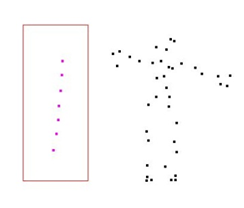
\includegraphics[width=3.6in]{segmentInitInverted.png}
\caption{Rope marker selection.}
\label{fig:SegInit} 
\end{figure}

As in Section \ref{secClustering}, at each frame we attempt to find a provisional marker location that is in close proximity to the next estimated position for a marker trace. When no provisional marker location can be found for a trace, instead of labeling a gap, we create a temporary marker for the marker trace. The temporary marker allows the algorithm to continue tracking a marker despite the presence of noise and gaps in the motion capture data.

In order to track a marker, we match provisional markers to traces using a linear combination of two predicted positions, $V_j^i$ and $N_j^i$. The first predicted position, $V_j^i$, is based on the last known velocity of the marker using equations (\ref{eq:1}), (\ref{eq:2}), and (\ref{eq:3}). The other position, $N_j^i$, is predicted using a midpoint displacement method, as described in Section \ref{sec:Gaps}, using equation (\ref{eq:6})--(\ref{eq:9}).

Then $V_j^i$ and $N_j^i$ are combined as follows:

\begin{equation}
F_j^i= \alpha V_j^i + (1 - \alpha) N_j^i,
\end{equation}

where $\alpha$ is one over the number of consecutive temporary markers. This means that the more consecutive temporary markers the trace has the less we rely on $V_j^i$, because it could have strayed too far from the actual rope markers. After fully segmenting the rope markers from the human markers it is possible to reconstruct the motion streams for each independently.

\section{Results} 

We present results that indicate that, under the assumption that the rope does not stretch, rope motion can be plausibly reconstructed from passive optical motion capture data without a physical model of rope dynamics.  This can be done in the presence of a human actor whose motion is tracked in the same capture session.  

Figure~\ref{fig:jumpRopeResult} shows the reconstruction of a motion capture session in which the character is jumping rope. Comparison with still frames taken during the capture session shows that both the marker segmentation and reconstruction algorithms accurately reproduce the original motion.

\begin{figure}[tb]
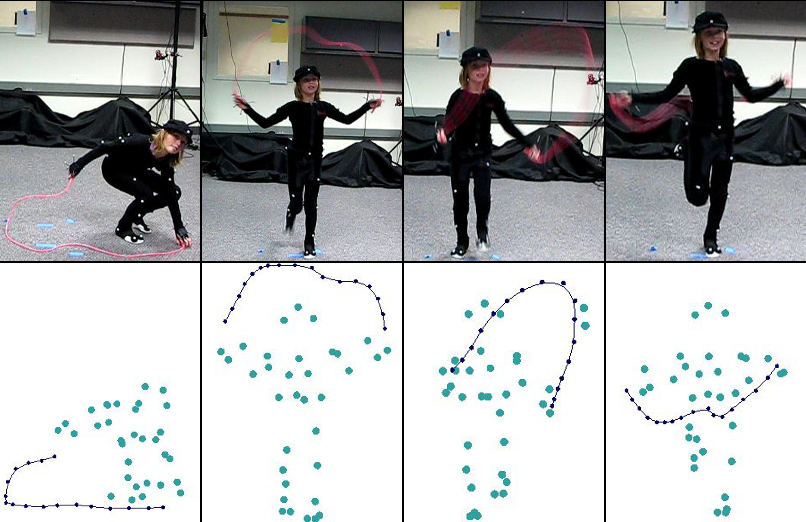
\includegraphics[width=\columnwidth]{jumpRopeFig.png}
\caption[Screenshots of original and reconstructed rope and human actor.]{Screenshots of the original motion, segmented rope and character markers, and the reconstructed rope with the human markers.}
\label{fig:jumpRopeResult} 
\end{figure}

Gap filling results in motion that is similar to missing motion in both magnitude and direction and has good continuity with surrounding motion.  Figure~\ref{fig:gapFillAnalysis} shows the average error for reconstructed marker positions for gaps created by holding back data from a motion capture session.  The horizontal axis shows the gap size in frames and the vertical axis shows the mean error for all frames in gaps of that size.  The data in Figure \ref{fig:gapFillAnalysis} were generated from 5,000 randomly generated gaps.  The curve is not smooth because of the random factors we included in the analysis. A gap created at different phases of a motion path might produce different values of error.

\begin{figure}[tb]
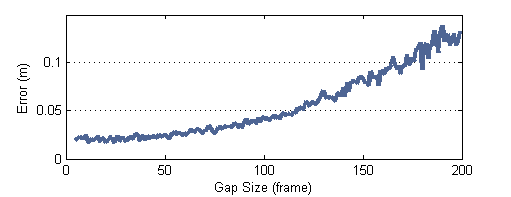
\includegraphics[width=\columnwidth]{gapAnalysisEasy50002.png}
\caption[Analysis of gap filling algorithm.]{Analysis of gap-filling algorithm. The horizontal axis is gap size and the vertical axis is error, which is the difference between the motion captured data after clustering and the data estimated by our method.}
\label{fig:gapFillAnalysis} 
\end{figure}

Figure~\ref{fig:Result} compares the original shape of the model with our results.  In the top row of Figure \ref{fig:Result}(a), we compare the ground truth motion data (left) with data generated by the gap-filling algorithm (right). The data shown in dash-dots on the left and right sides of each image is held back during gap filling. The synthesized motion, which is the bottom marker in solid lines on the right image of (a), preserves good continuity with existing motion and rope shape. Figure \ref{fig:Result}(b) shows traces (right) created from raw point cloud (left).

The process accurately extracts motion in a variety of settings.  Still images from both video taken during a capture session and reconstructed motion from that session are shown in Figure \ref{fig:Result}(c)--(f).  Each scenario is described subsequently, and complete video clips are included as reference material with this paper.

Five dangling ropes, as shown in Figure \ref{fig:Result}(c), have one end fixed to a horizontal support bar and rope motion is driven by hitting the ropes with a stick. This scenario is easy to process because one end of the rope is anchored to a fixed position in space and rope motions are relatively small. The resulting motion is smooth with few gaps and little noise.

We recorded a rope dropping from the horizontal support bar (shown in Figure \ref{fig:Result}(d)). The rope has one end fixed to the bar.  The rope is nudged over the edge of the bar using a stick.  This scenario is more complex than the five dangling ropes because the rope moves more quickly and with more bending.  We processed this data in inverse time order, so the structure of dangling rope is clearer at the end than at the beginning of the session . 

The motion of unanchored ribbons is more difficult to process because ribbons have less mass and are not anchored in this example.  Figure \ref{fig:Result}(e) and (f) show two frames from two sessions involving ribbons attached to a wand that is waved freely in the capture arena.  Ribbon is also more difficult because it is a lighter material that accelerates with less force than rope. By mapping different textures to the single ribbon motion, we create some interesting effects, such as animating lace cloth and a Japanese fish flag based on captured data.

\begin{figure}[tb]
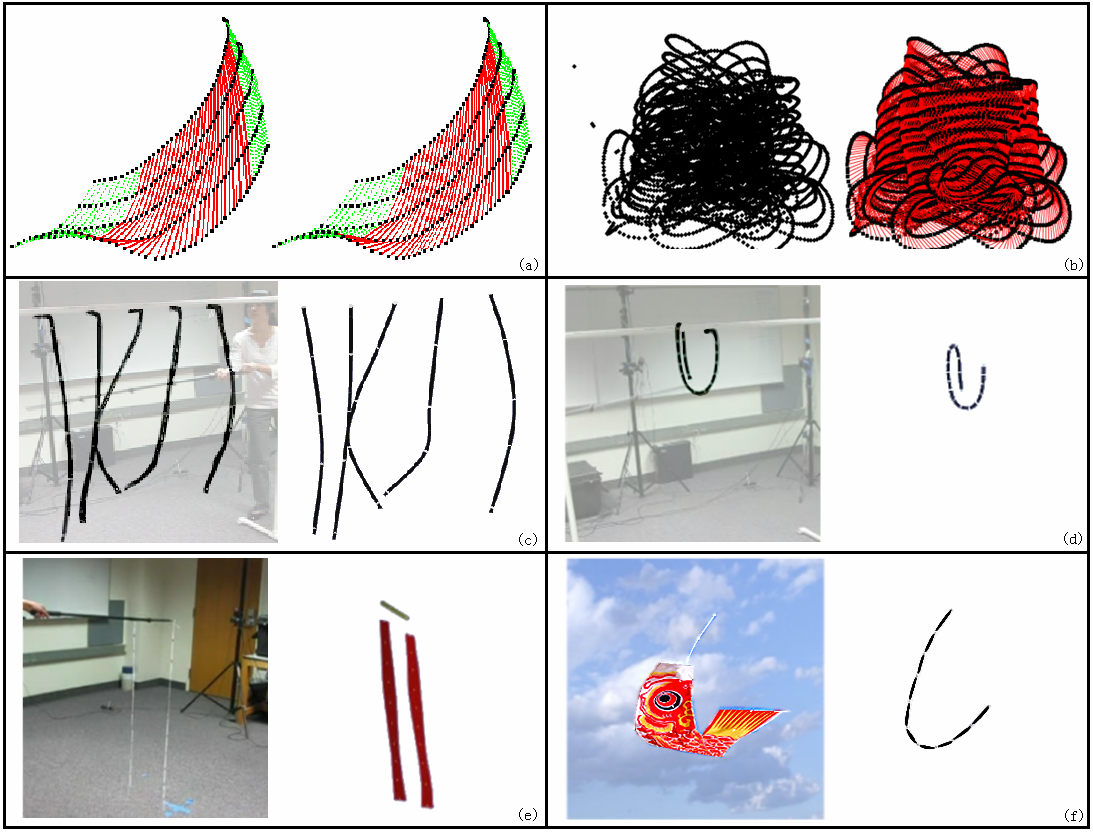
\includegraphics[width=\columnwidth]{result.png}
\caption{Screenshots of reconstructed motion of ropes and ribbon.}
\label{fig:Result} 
\end{figure}

\section{Conclusion and Discussion} 

Our work produces visually plausible rope motion from passive optical motion capture data using a statistical model under the assumption that the rope does not stretch.  The algorithm uses a novel clustering scheme, forward differencing, and a recursive midpoint scheme to automatically detect and remove most noise, gaps, and marker swaps.  The algorithm preserves continuity of motion in traces and fits the shape of rope.  This work lays a foundation for further investigation of motion capture for non-rigid bodies using statistical rather than physical models.  The approach to the problem may advance motion capture results for non-rigid bodies driven by complex or poorly understood physical systems.

Complicated motions (such as spirals, collisions, sudden changes in movement, or extremely fast movement) are not well handled in this model. Our assumptions for detecting swaps may be oversimplified relative to natural movement. Consideration of other factors, such as velocity or acceleration, might improve gap-filling results.  We have used a simple method for interpolating rope position between markers.  More complex methods may result in more plausible results particularly when the distance between markers on the rope is large.  
